\documentclass[a4paper,10.5pt]{ltjsarticle}
\usepackage{graphicx}
\usepackage{graphics}
\usepackage{luatexja-fontspec}
\usepackage{caption}
\usepackage{amsmath,amssymb,bm,braket}
\usepackage{gnuplot-lua-tikz}
\usepackage[top=10truemm,bottom=15truemm,left=10truemm,right=10truemm]{geometry}
\usepackage{array}
\usepackage{upgreek}
\usepackage{fancyhdr}
\renewcommand{\refname}{}
\usepackage{listings,jvlisting} %日本語のコメントアウトをする場合jvlisting(もしくはjlisting)が必要
%ここからソースコードの表示に関する設定
\lstset{
  basicstyle={\ttfamily},
  identifierstyle={\small},
  commentstyle={\smallitshape},
  keywordstyle={\small\bfseries},
  ndkeywordstyle={\small},
  stringstyle={\small\ttfamily},
  frame={tb},
  breaklines=true,
  columns=[l]{fullflexible},
  numbers=left,
  xrightmargin=0pt,
  xleftmargin=3pt,
  numberstyle={\scriptsize},
  stepnumber=1,
  numbersep=1pt,
  lineskip=-0.5ex
}
\captionsetup[figure]{format=plain, labelformat=simple, labelsep=quad, font=bf}
\captionsetup[table]{format=plain, labelformat=simple, labelsep=quad, font=bf}
\parindent = 0pt
\setmainjfont[BoldFont=HiraMinProN-W6]{HiraMinPro-W3}
\begin{document}
\centerline
{\huge \bfseries E2 予習課題}
{\bfseries 62115799 \\平井優我}\\
\\
\leftline
{\Large \bfseries 1.理論}
 今回の実験ではBall\&Beam実験装置を用いて実験を行う。図1にフィードバックシステムの図を示す。
\begin{figure}[h]
  \centering
  \includegraphics[scale=0.3]{figure1.eps}
  \caption{フィードバックシステム}
\end{figure}
\\
{\large \bfseries 1.1 離散時間状態方程式の導出}\\
 制御対象である実験装置について、サーボモーターへの印加電圧を$v$、それによってボールの位置$z$や速度$\dot{z}$、サーボモーターの角度$\theta$や角速度$\dot{\theta}$が駆動される入出力システムである。ここで、$u_\mathrm{c}(t)=v(t)\ ,\ \bm x(t)=[\theta,\dot{\theta},z,\dot{z}]^\top$とおく。また、センサーを用いて全状態を観測できるとすると、観測信号$\bm y_\mathrm{c}(t)$は$\bm x(t)$そのものとなる。システム$P_\mathrm{c}$は次のように表せる。

\begin{equation}
  P_\mathrm{c}:\dot{\bm x}(t)=A_\mathrm{c}\bm x (t)+B_\mathrm{c}u_\mathrm{c}(t)\ ,\ \bm y_\mathrm{c}=\bm x(t)
\end{equation}

ここで、$A_\mathrm{c}\in \mathbb{R}^{4\times4},B_\mathrm{c}\in \mathbb{R}^4$である。\\
 計算機を用いて信号を処理する場合、装置から得られた連続時間信号をホールダとサンプラを用いて離散時間信号に変換しなければならない。サンプラのサンプリング周期を$\Delta t$とすると、$t=k\Delta t\ ,\ \forall k\in\{0,1,2,3\cdots\}$という離散時間毎に$\bm y_\mathrm{c}$の値を取得することになる。得られた数列を$\bm y_\mathrm{c}[k]$のように離散時間$[k]$をつけて表記すると、

\begin{equation}
  \bm y_\mathrm{c}[k]=\bm y_\mathrm{c}(k\Delta t)\ ,\ \forall k\in\{0,1,2,3\cdots\}
\end{equation}

の関係が成り立つ。次に今回の実験ではホールダについて0次ホールドを用いる。よって、信号$u_\mathrm{c}(t)$はある時刻$t=k\Delta t$から$t=(k+1)\Delta t$までの間は$u[k]$の一定値をとる。すなわち、

\begin{equation}
  u_\mathrm{c}(t)=u[k]\ ,\ \forall t\in[k\Delta t,(k+1)\Delta t]\ ,\ \forall k\in\{0,1,2,3\cdots\}
\end{equation}

の関係が成り立つ。\\
 これより、$P_\mathrm{c}$、サンプラ、ホールダのモデルをもとにして、$u[k]$から$y[k]$までの振る舞いをモデル化する。まず、(1)式の連続時間状態方程式で、時間$t=k\Delta t$からサンプリング周期が一個先の$t=(k+1)\Delta t$までの状態$\bm x(t)$の遷移を計算すると、
\begin{equation}
  \bm x((k+1)\Delta t)=e^{A_\mathrm{c}\Delta t}+\int_{k\Delta t}^{(k+1)\Delta t} e^{A_\mathrm{c}((k+1)\Delta t-\tau)}B_\mathrm{c}u_\mathrm{c}(\tau)\mathrm{d}\tau
\end{equation}

となる。ここで、(3)式と$\tau=(k+1)\Delta t-\tau$と置き直すことによって(4)式は、

\begin{equation}
  \bm x((k+1)\Delta t)=e^{A_\mathrm{c}\Delta t}+\left\{\int_{0}^{\Delta t} e^{A_\mathrm{c}\tau}B_\mathrm{c}\mathrm{d}\tau\right\}u_\mathrm{c}(\tau)
\end{equation}

と書き換えることができる。さらに、サンプリング周期に合わせた$t=k\Delta t\ ,\ k\in\{0,1,2,3\cdots\}$の離散時間上の状態$\bm x(t)$を$\bm x[k]$と表記する。このとき、(2)式のように$\bm x[k]=\bm x(k\Delta t)\ ,\ k\in \{0,1,2,3\cdots\}$が成り立つため、$u[k]$から$y[k]=x[k]$までの振る舞いは、

\begin{equation}
  \mathrm{P}:\bm x[k+1]=A\bm x[k]+Bu[k]
\end{equation}

と記述できる。ただし、$A\in \mathbb{R}^{4\times4}$と$B\in \mathbb{R}^{4}$はそれぞれ、

\begin{equation}
  A=e^{A_\mathrm{c}\Delta t}\ ,\ B=\int_{0}^{\Delta t}e^{A_\mathrm{c}\tau}\mathrm{d}\tau
\end{equation}

とした。
 以上より、離散時間状態方程式では逐次代入をするだけで振る舞いを計算することができる。初期状態が$\bm x[0]=\bm x_0$であるとすると、入力信号$\{u[0]u[1]\cdots u[k-1]\}$のもとで$\bm x[k]$は、

\begin{equation}
  \bm x[k]=A^k\bm x_0+\sum^{k-1}_{\tau=0}A^{\tau}Bu[k-1-\tau]
\end{equation}

のように求めることができる。\\
\\
{\Large \bfseries 演習課題1}\\
{\large \bfseries 1.テキストを参考に離散時間状態方程式 (4) を導出してみよう.}\\
 上で求めた。\\
\\
{\large \bfseries 2.\ Python で関数 ss を用いて動的システムを状態方程式で記述してみよう.たとえば,2 次元の状態方
程式を一つ何でも考えてみよう.以下では,この状態方程式を sys と名付ける.}\\

\begin{lstlisting}
   A = np.array([[0.99877083, 0.04875026], [-0.04875026, 0.95002057]])
   B = np.array([[0.00122917],[0.04875026]])
   C = np.array([[1, 0]])
   D = np.array([0])
   st = 0.05 # サンプリング周期
  sys = ss(A, B, C, D, st) # 離散時間状態方程式
\end{lstlisting}

{\large \bfseries 3.Python で関数 impulse や step を用いて sys のインパルス応答やステップ応答を計算し,描画してみよう.また,手計算で計算した結果と一致することを確認しよう.}\\

\begin{figure}[h]
  \centering
  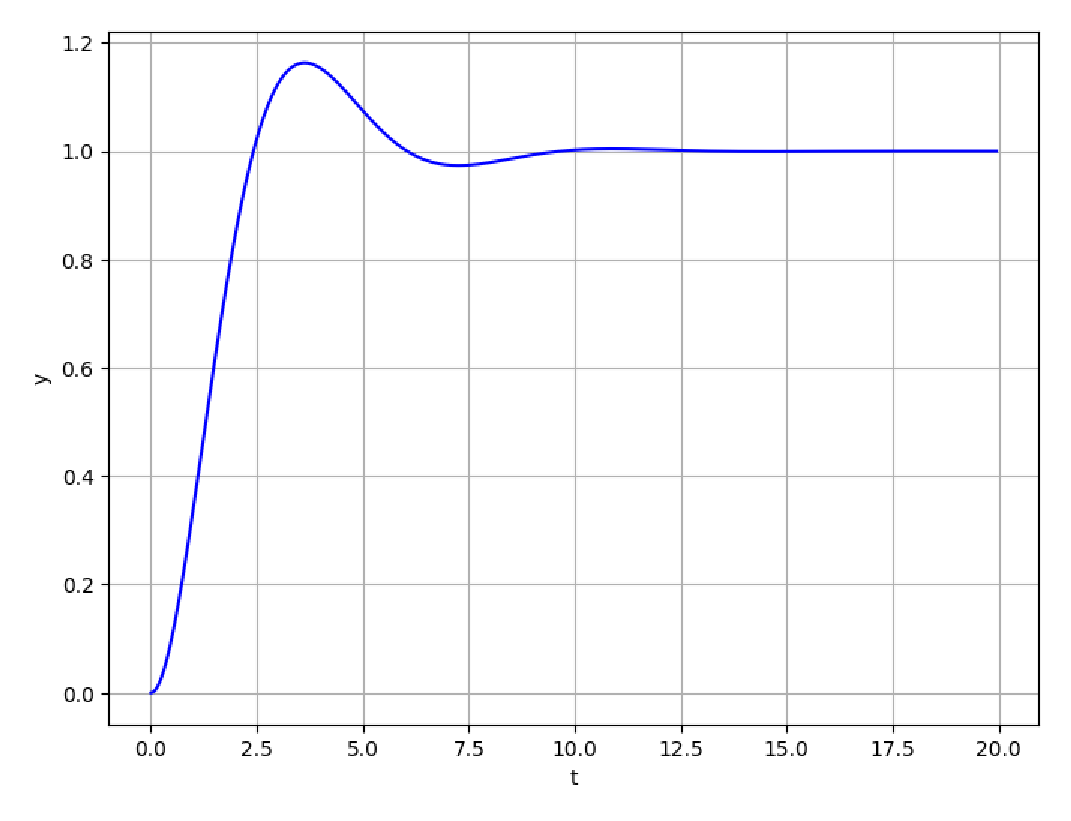
\includegraphics[scale=0.5]{figure2.eps}
  \caption{ステップ応答}
\end{figure}

\begin{figure}[h]
  \centering
  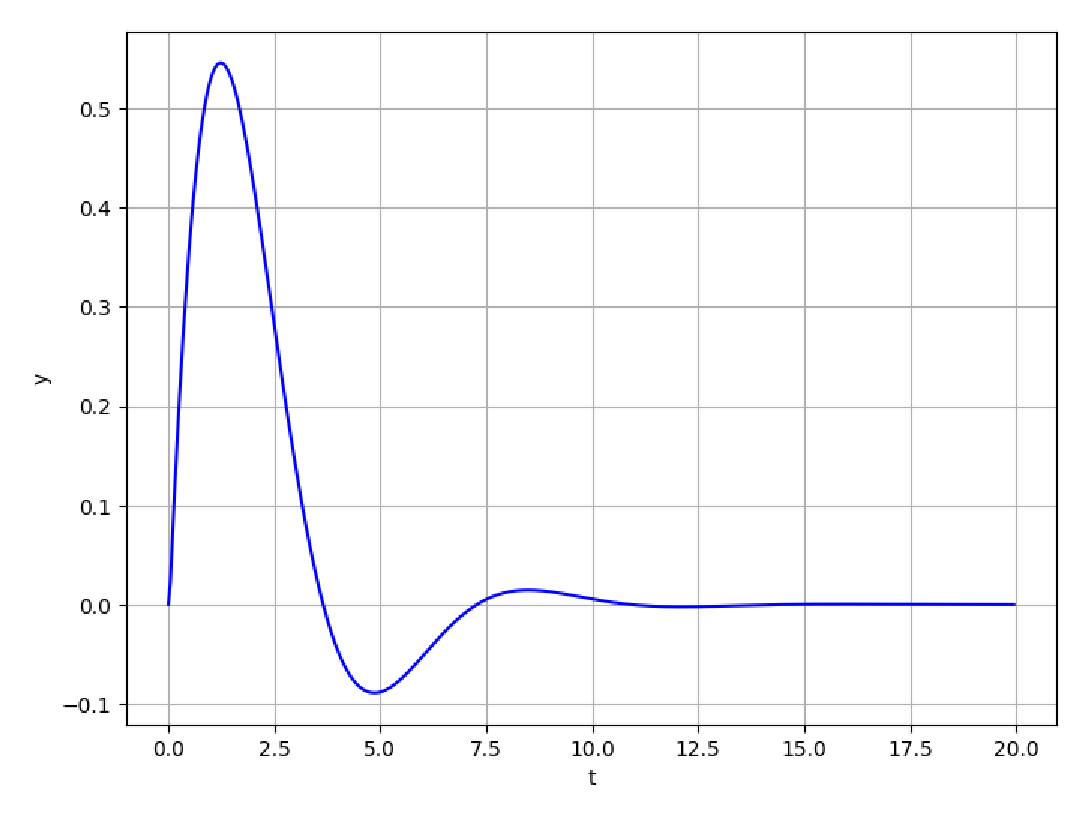
\includegraphics[scale=0.5]{figure3.eps}
  \caption{インパルス応答}
\end{figure}

{\Large \bfseries 演習課題2}\\
{\large \bfseries 1.適当な状態方程式を定義して,ステップ応答のデータを集めてみよう.そして,データから状態方程式 を再構成できることを確認してみよう.}\\
\centerline{実行プログラム}
\begin{lstlisting}
   x = np.array([[0], [0]]) # 初期状態
   u = 1.0 # ステップ信号
   x1_data = [] # 状態1を保存
   x2_data = [] # 状態2を保存
   u_data = [] # 入力を保存
   t_data = [] # 時間を保存
   for t in np.arange(0,Tend,st):
      x1_data.append(x[0,0]) # データへの格納
      x2_data.append(x[1,0])
      u_data.append(u)
      t_data.append(t)
      x = A @ x + B * u # 状態方程式による状態の更新
   Avar = cp.Variable((2, 2)) # 行列変数の定義
   Bvar = cp.Variable((2, 1))
   x1_array = np.array(x1_data) # 型の変換
   x2_array = np.array(x2_data)
   X1 = np.array([x1_array[1:],x2_array[1:]]) # データ行列の定義
   X0 = np.array([x1_array[:-1],x2_array[:-1]])
   U0 = np.array([u_data[:-1]])
   error = X1 - (Avar @ X0 + Bvar @ U0) # 評価関数の設定
   objective = cp.norm(error, "fro") # フロベニウスノルム
   prob = cp.Problem(cp.Minimize(objective)) # 最小化問題
   prob.solve(verbose=False)
   print(Avar.value) # 結果の表示
   print(Bvar.value)
\end{lstlisting}
\centerline{実行結果}
\begin{lstlisting}
  [[ 0.99877083  0.04875026]
   [-0.04875026  0.95002057]]
  [[0.00122917]
   [0.04875026]]
\end{lstlisting}
\centerline{ }
{\large \bfseries 2.1 のステップ応答に観測ノイズが加わったとして,もう一度,状態方程式を再構成できることを確認してみよう.ノイズの大きさを変えて色々と検証してみよう.}\\

\centerline{実行プログラム}
\begin{lstlisting}
   x = np.array([[0], [0]]) # 初期状態
   u = 1.0 # ステップ信号
   x1_data = [] # 状態1を保存
   x2_data = [] # 状態2を保存
   u_data = [] # 入力を保存
   t_data = [] # 時間を保存
   for t in np.arange(0,Tend,st):
      x1_data.append(x[0,0]) # データへの格納
      x2_data.append(x[1,0])
      u_data.append(u)
      t_data.append(t)
      x = A @ x + B * u # 状態方程式による状態の更新
      x = x + 0.01*np.random.randn(2,1) # 観測ノイズの追加
   Avar = cp.Variable((2, 2)) # 行列変数の定義
   Bvar = cp.Variable((2, 1))
   x1_array = np.array(x1_data) # 型の変換
   x2_array = np.array(x2_data)
   X1 = np.array([x1_array[1:],x2_array[1:]]) # データ行列の定義
   X0 = np.array([x1_array[:-1],x2_array[:-1]])
   U0 = np.array([u_data[:-1]])
   error = X1 - (Avar @ X0 + Bvar @ U0) # 評価関数の設定
   objective = cp.norm(error, "fro") # フロベニウスノルム
   prob = cp.Problem(cp.Minimize(objective)) # 最小化問題
   prob.solve(verbose=False)
   print(Avar.value) # 結果の表示
   print(Bvar.value)
\end{lstlisting}
\centerline{実行結果}
\begin{lstlisting}
  [[ 0.9956988   0.04454225]
   [-0.05717894  0.93833348]]
  [[0.00440052]
   [0.05665428]]
\end{lstlisting}
\centerline{ }
{\large \bfseries 3.事前情報を取り入れたデータ駆動モデリングにも取り組んでみよう.}\\
 $k+1$と$k$の位置の変位は速度とサンプリング周期の積で表され、また、速度を入力によって制御すると考える。
\centerline{状態方程式}
\begin{lstlisting}
  st = 0.05 # サンプリング周期
  A = np.array([[1, st], [0, 1]])
  B = np.array([[0],[0.04875026]])
  C = np.array([[1, 0]])
  D = np.array([0])
  sys = ss(A, B, C, D, st) # 離散時間状態方程式
\end{lstlisting}

\begin{figure}[h]
  \centering
  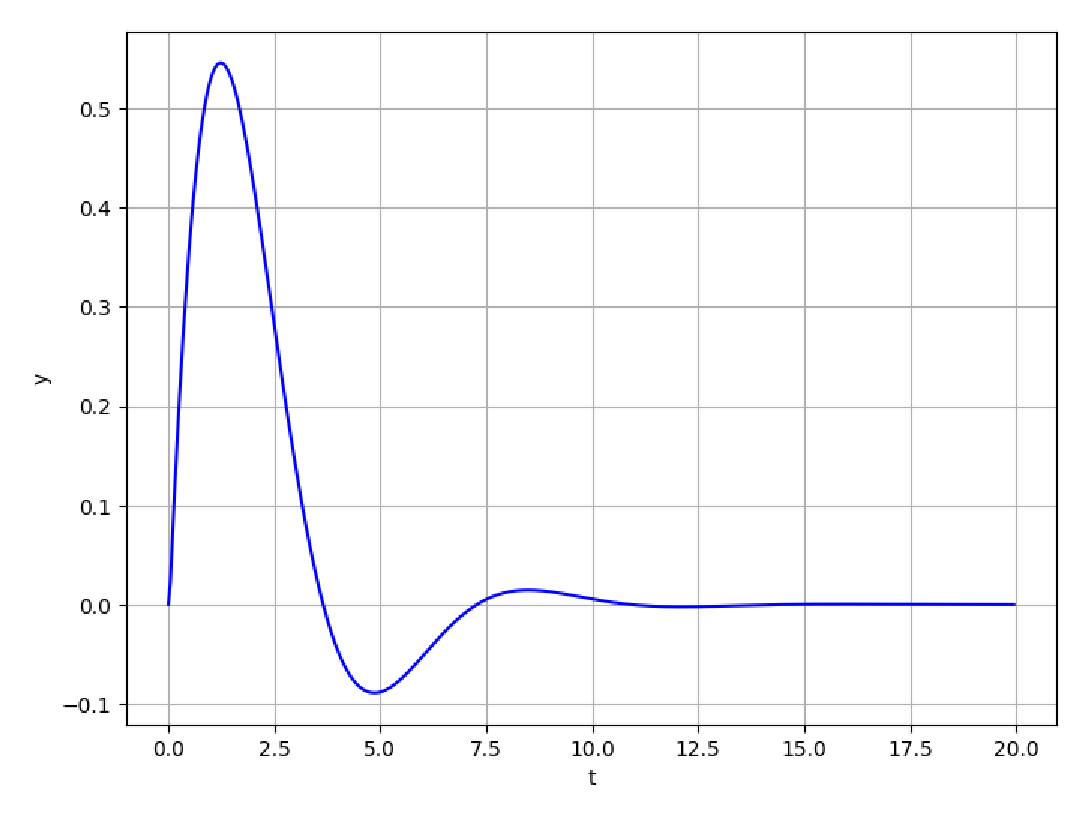
\includegraphics[scale=0.5]{figure3.eps}
  \caption{ステップ応答}
\end{figure}
\clearpage
\begin{figure}[h]
  \centering
  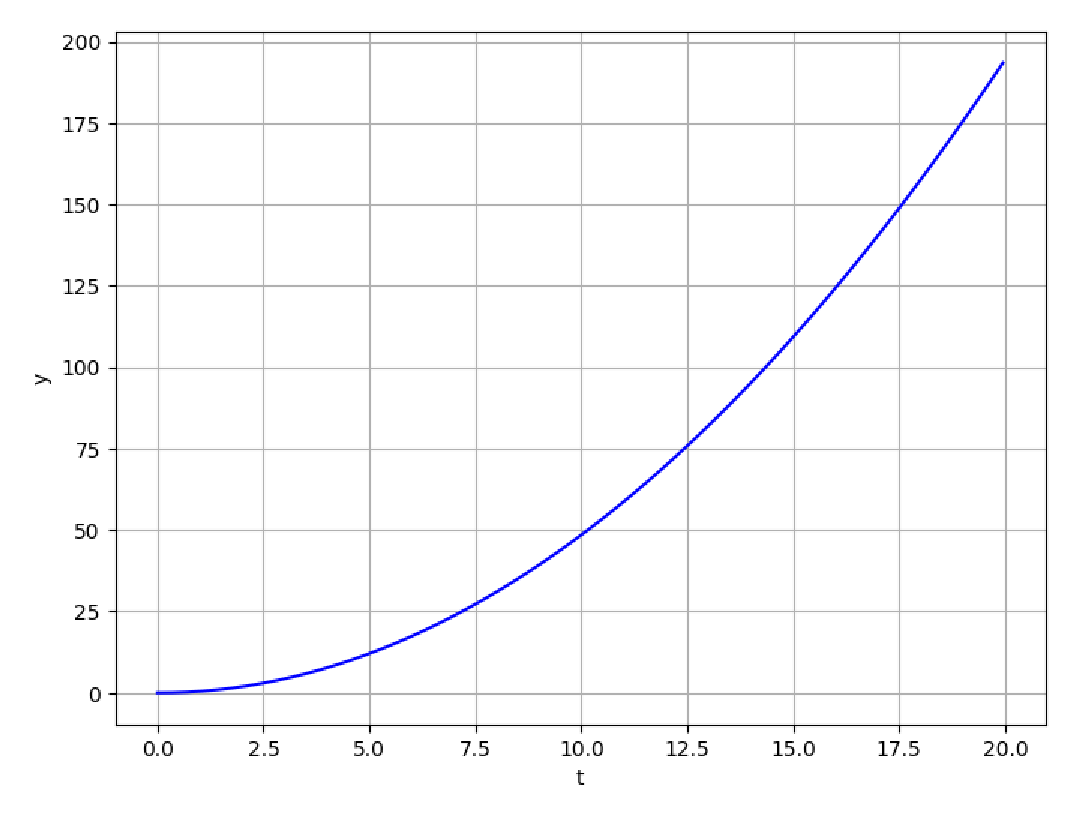
\includegraphics[scale=0.5]{figure4.eps}
  \caption{インパルス応答}
\end{figure}

\centerline{ノイズなしでの再構成}
\begin{lstlisting}
  [[ 1.00000000e+00  5.00000000e-02]
   [-1.48135268e-17  1.00000000e+00]]
  [[-3.25512585e-15]
   [ 4.87502600e-02]]
\end{lstlisting}

\centerline{ノイズありでの再構成}
\begin{lstlisting}
  [[1.00058631 0.04276865]
   [0.00102313 0.98851602]]
  [[0.00239231]
   [0.00825118]]
\end{lstlisting}
\centerline{ }
{\Large \bfseries 演習課題3}\\
{\large \bfseries 1.テキストを参考に離散時間状態方程式 (4) を導出してみよう.}\\

{\large \bfseries 2.実データを用いて$\mathrm{P_{up}}$のシステム行列$A_\mathrm{up}$と$B_\mathrm{up}$を求めよ.その際に,どのような同定信号を用いることが望ましいか,上流システムに関する事前情報はどのようなものがあるか,また事前情報をどのように取り入れるべきか,もよく検討してみよう.}\\

\centerline{$A_\mathrm{up},B_\mathrm{up}$の同定}
\begin{lstlisting}
  [[1.00058631 0.04276865]
   [0.00102313 0.98851602]]
  [[0.00239231]
   [0.00825118]]
\end{lstlisting}

{\large \bfseries 3. 2で得られた$\mathrm{P_{up}}$と物理法則から得られる$\mathrm{P_{down}}$を用いて全体の状態方程式モデル(4)を構築して,
Python を用いてインパルス応答のシミュレーションをせよ.}\\

\begin{figure}[h]
  \centering
  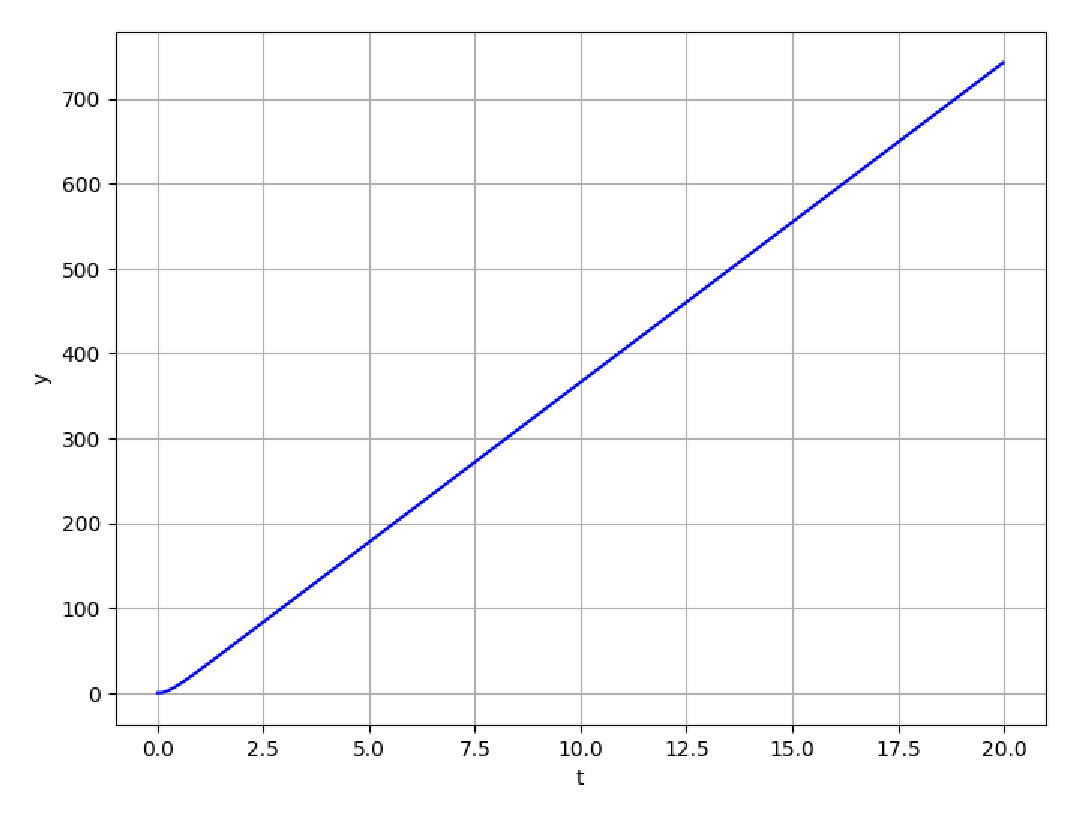
\includegraphics[scale=0.5]{figure6.eps}
  \caption{$z$のインパルス応答}
\end{figure}

\begin{figure}[h]
  \centering
  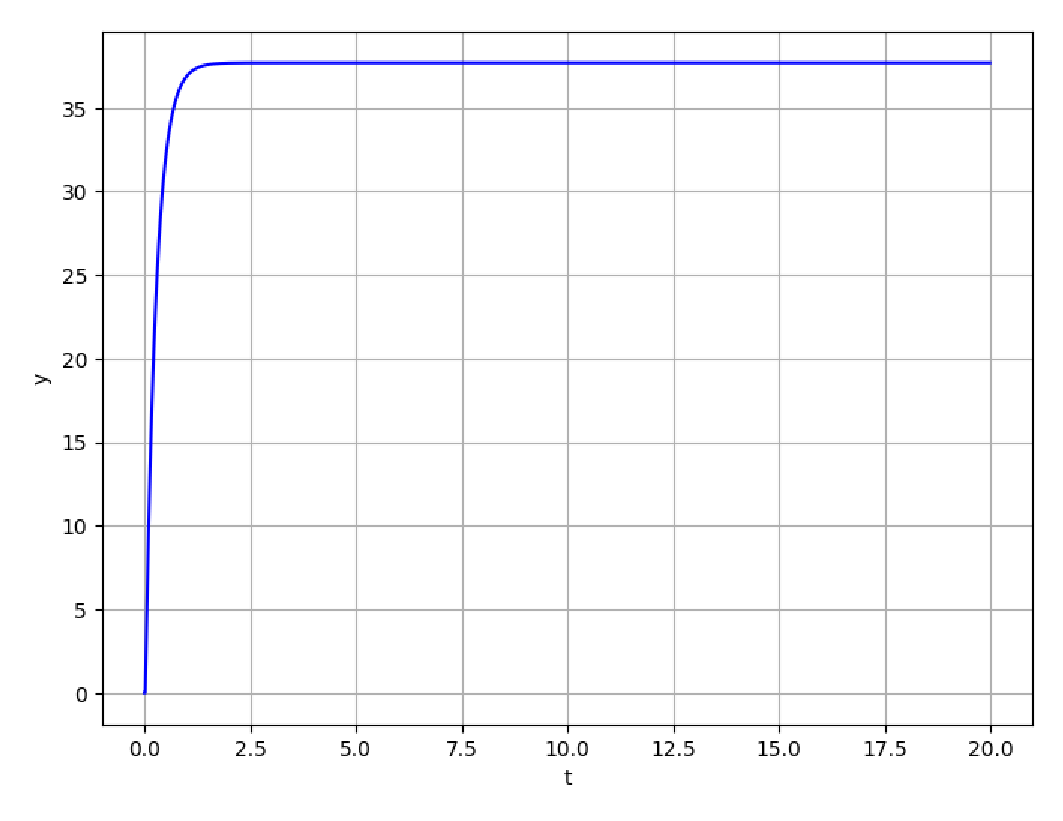
\includegraphics[scale=0.5]{figure7.eps}
  \caption{$v_z$のインパルス応答}
\end{figure}

\begin{figure}[h]
  \centering
  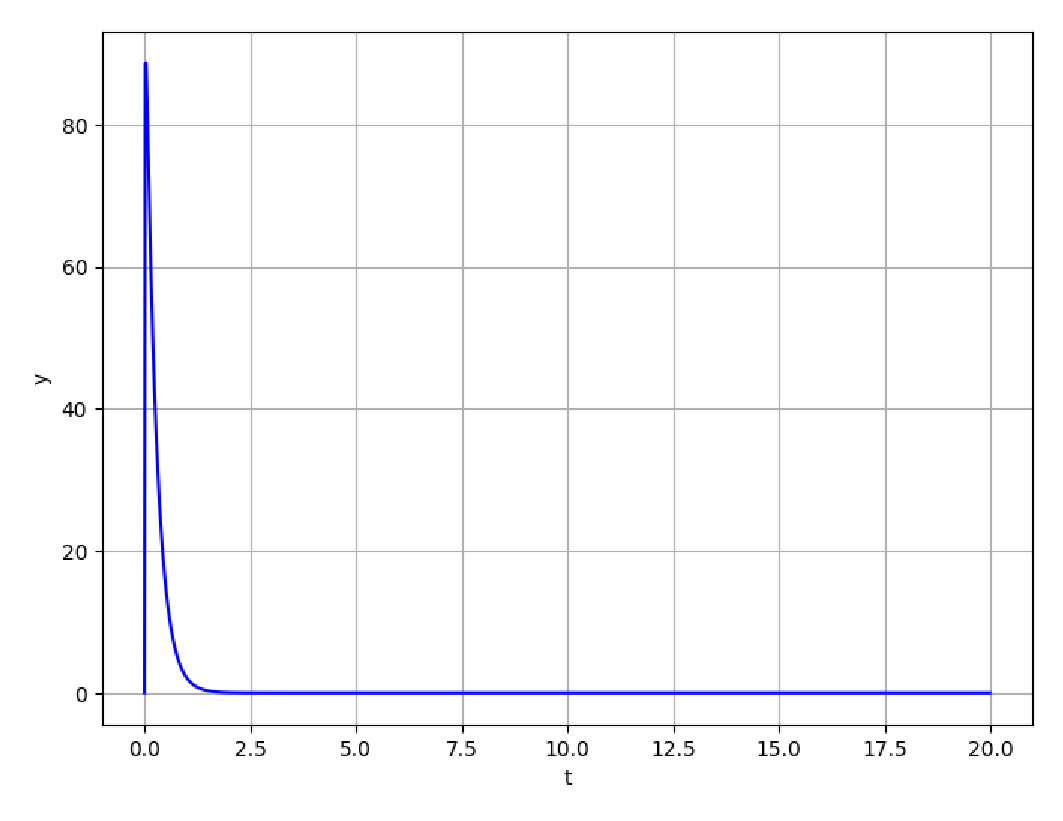
\includegraphics[scale=0.5]{figure8.eps}
  \caption{$\theta$のインパルス応答}
\end{figure}

\begin{figure}[h]
  \centering
  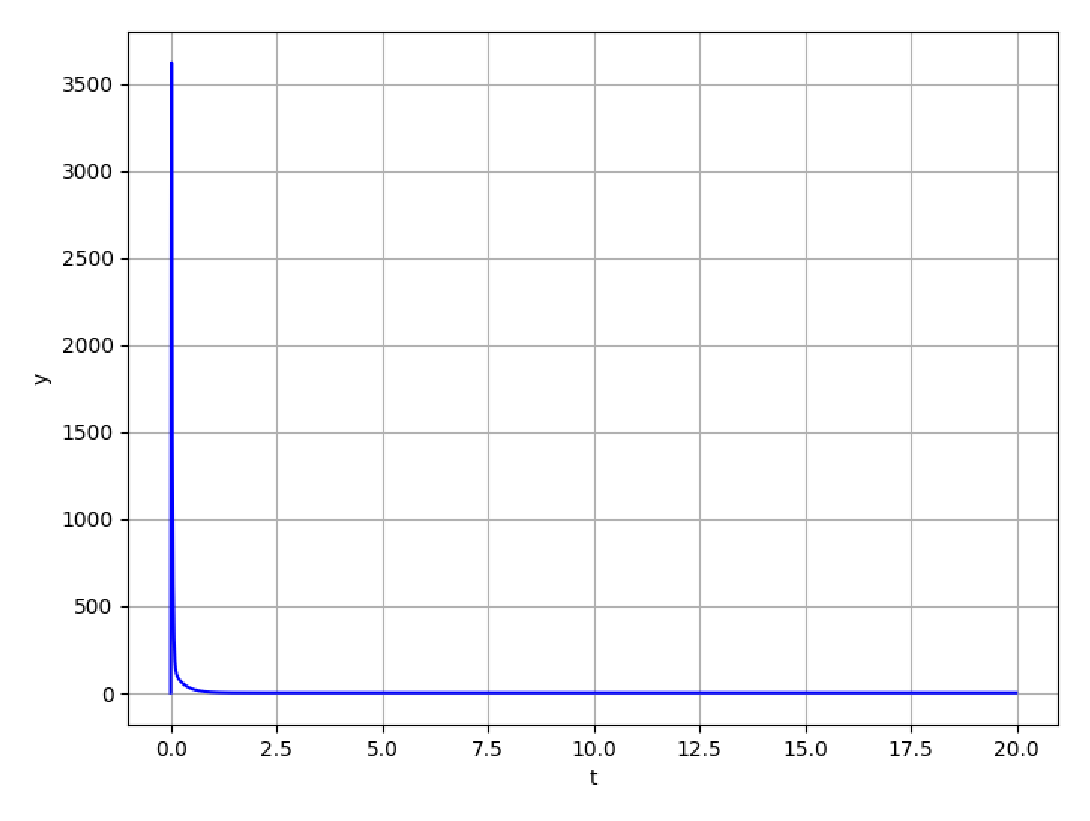
\includegraphics[scale=0.5]{figure9.eps}
  \caption{$\dot{\theta}$のインパルス応答}
\end{figure}




\end{document}
